\documentclass[1p]{elsarticle_modified}
%\bibliographystyle{elsarticle-num}

%\usepackage[colorlinks]{hyperref}
%\usepackage{abbrmath_seonhwa} %\Abb, \Ascr, \Acal ,\Abf, \Afrak
\usepackage{amsfonts}
\usepackage{amssymb}
\usepackage{amsmath}
\usepackage{amsthm}
\usepackage{scalefnt}
\usepackage{amsbsy}
\usepackage{kotex}
\usepackage{caption}
\usepackage{subfig}
\usepackage{color}
\usepackage{graphicx}
\usepackage{xcolor} %% white, black, red, green, blue, cyan, magenta, yellow
\usepackage{float}
\usepackage{setspace}
\usepackage{hyperref}

\usepackage{tikz}
\usetikzlibrary{arrows}

\usepackage{multirow}
\usepackage{array} % fixed length table
\usepackage{hhline}

%%%%%%%%%%%%%%%%%%%%%
\makeatletter
\renewcommand*\env@matrix[1][\arraystretch]{%
	\edef\arraystretch{#1}%
	\hskip -\arraycolsep
	\let\@ifnextchar\new@ifnextchar
	\array{*\c@MaxMatrixCols c}}
\makeatother %https://tex.stackexchange.com/questions/14071/how-can-i-increase-the-line-spacing-in-a-matrix
%%%%%%%%%%%%%%%

\usepackage[normalem]{ulem}

\newcommand{\msout}[1]{\ifmmode\text{\sout{\ensuremath{#1}}}\else\sout{#1}\fi}
%SOURCE: \msout is \stkout macro in https://tex.stackexchange.com/questions/20609/strikeout-in-math-mode

\newcommand{\cancel}[1]{
	\ifmmode
	{\color{red}\msout{#1}}
	\else
	{\color{red}\sout{#1}}
	\fi
}

\newcommand{\add}[1]{
	{\color{blue}\uwave{#1}}
}

\newcommand{\replace}[2]{
	\ifmmode
	{\color{red}\msout{#1}}{\color{blue}\uwave{#2}}
	\else
	{\color{red}\sout{#1}}{\color{blue}\uwave{#2}}
	\fi
}

\newcommand{\Sol}{\mathcal{S}} %segment
\newcommand{\D}{D} %diagram
\newcommand{\A}{\mathcal{A}} %arc


%%%%%%%%%%%%%%%%%%%%%%%%%%%%%5 test

\def\sl{\operatorname{\textup{SL}}(2,\Cbb)}
\def\psl{\operatorname{\textup{PSL}}(2,\Cbb)}
\def\quan{\mkern 1mu \triangleright \mkern 1mu}

\theoremstyle{definition}
\newtheorem{thm}{Theorem}[section]
\newtheorem{prop}[thm]{Proposition}
\newtheorem{lem}[thm]{Lemma}
\newtheorem{ques}[thm]{Question}
\newtheorem{cor}[thm]{Corollary}
\newtheorem{defn}[thm]{Definition}
\newtheorem{exam}[thm]{Example}
\newtheorem{rmk}[thm]{Remark}
\newtheorem{alg}[thm]{Algorithm}

\newcommand{\I}{\sqrt{-1}}
\begin{document}

%\begin{frontmatter}
%
%\title{Boundary parabolic representations of knots up to 8 crossings}
%
%%% Group authors per affiliation:
%\author{Yunhi Cho} 
%\address{Department of Mathematics, University of Seoul, Seoul, Korea}
%\ead{yhcho@uos.ac.kr}
%
%
%\author{Seonhwa Kim} %\fnref{s_kim}}
%\address{Center for Geometry and Physics, Institute for Basic Science, Pohang, 37673, Korea}
%\ead{ryeona17@ibs.re.kr}
%
%\author{Hyuk Kim}
%\address{Department of Mathematical Sciences, Seoul National University, Seoul 08826, Korea}
%\ead{hyukkim@snu.ac.kr}
%
%\author{Seokbeom Yoon}
%\address{Department of Mathematical Sciences, Seoul National University, Seoul, 08826,  Korea}
%\ead{sbyoon15@snu.ac.kr}
%
%\begin{abstract}
%We find all boundary parabolic representation of knots up to 8 crossings.
%
%\end{abstract}
%\begin{keyword}
%    \MSC[2010] 57M25 
%\end{keyword}
%
%\end{frontmatter}

%\linenumbers
%\tableofcontents
%
\newcommand\colored[1]{\textcolor{white}{\rule[-0.35ex]{0.8em}{1.4ex}}\kern-0.8em\color{red} #1}%
%\newcommand\colored[1]{\textcolor{white}{ #1}\kern-2.17ex	\textcolor{white}{ #1}\kern-1.81ex	\textcolor{white}{ #1}\kern-2.15ex\color{red}#1	}

{\Large $\underline{12a_{0892}~(K12a_{0892})}$}

\setlength{\tabcolsep}{10pt}
\renewcommand{\arraystretch}{1.6}
\vspace{1cm}\begin{tabular}{m{100pt}>{\centering\arraybackslash}m{274pt}}
\multirow{5}{120pt}{
	\centering
	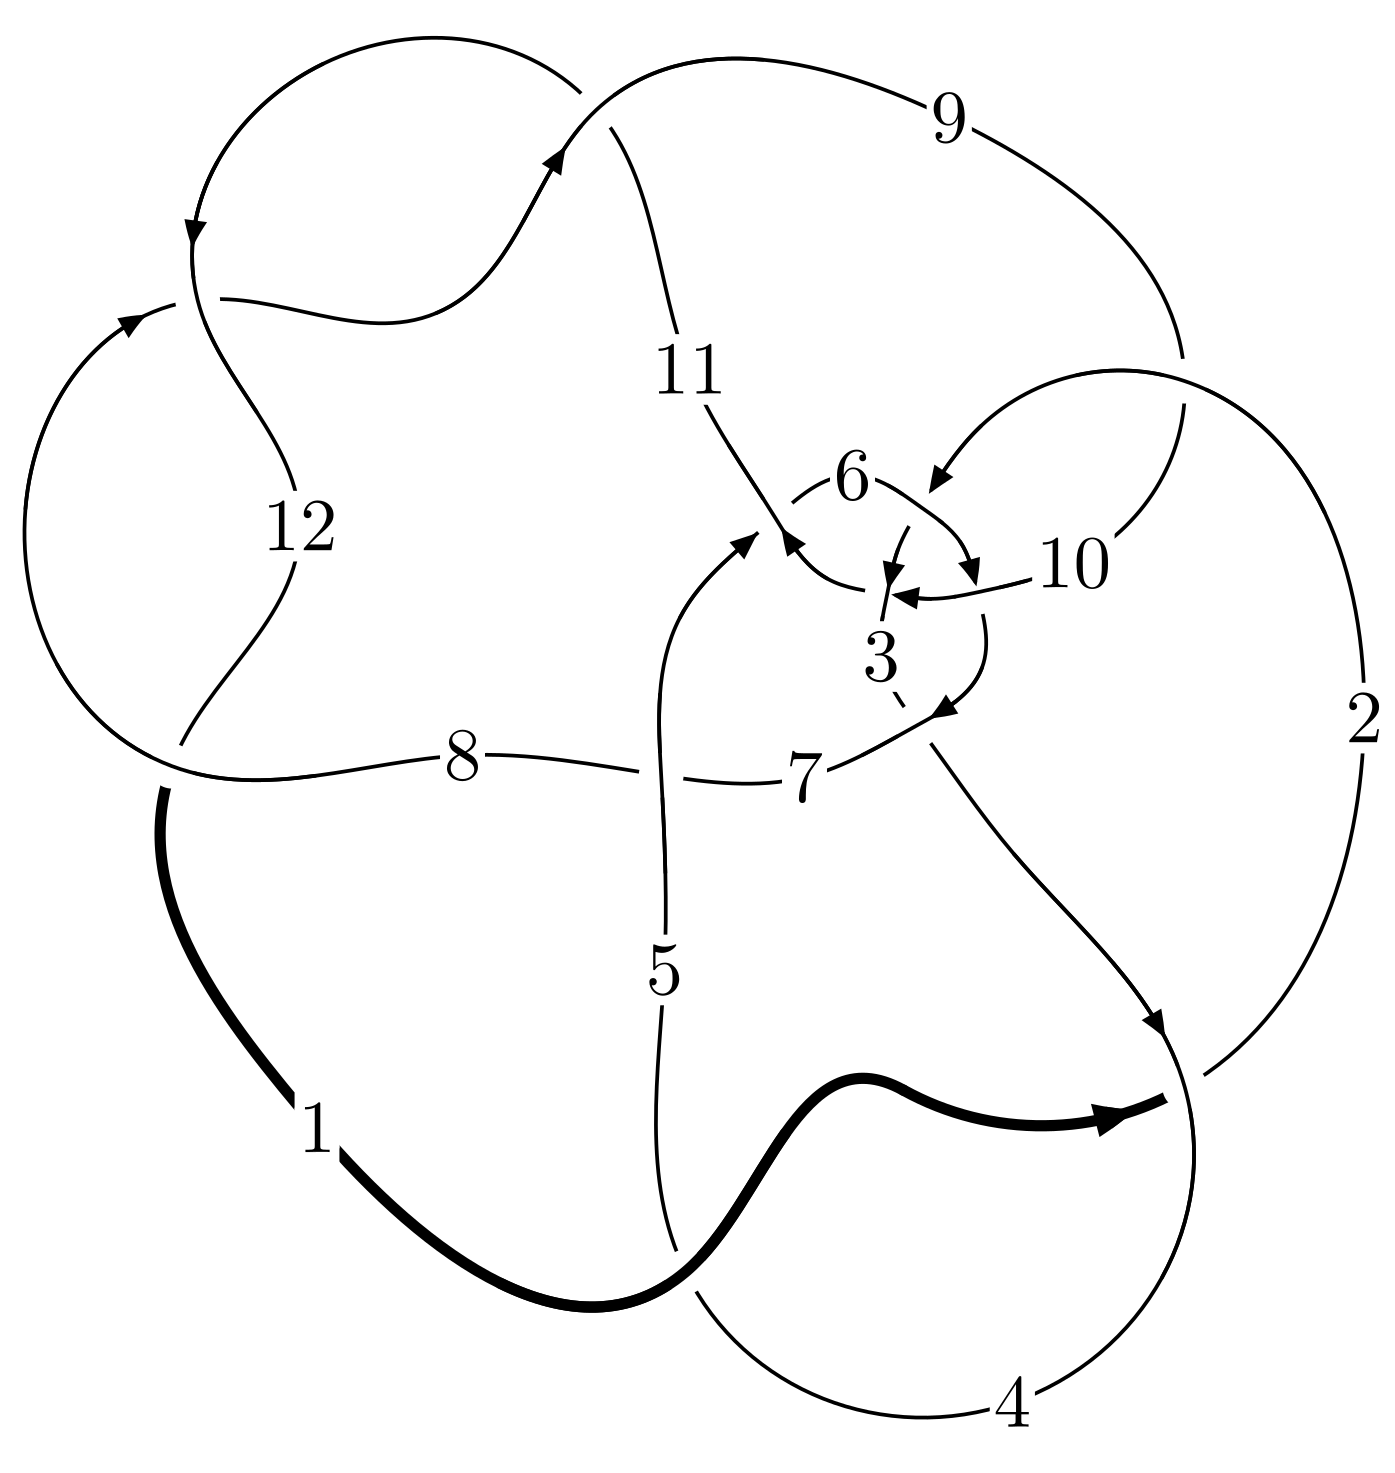
\includegraphics[width=112pt]{../../../GIT/diagram.site/Diagrams/png/1693_12a_0892.png}\\
\ \ \ A knot diagram\footnotemark}&
\allowdisplaybreaks
\textbf{Linearized knot diagam} \\
\cline{2-2}
 &
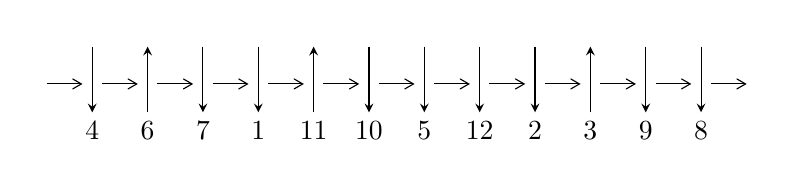
\begin{tikzpicture}[x=20pt, y=17pt]
	% nodes
	\node (C0) at (0, 0) {};
	\node (C1) at (1, 0) {};
	\node (C1U) at (1, +1) {};
	\node (C1D) at (1, -1) {4};

	\node (C2) at (2, 0) {};
	\node (C2U) at (2, +1) {};
	\node (C2D) at (2, -1) {6};

	\node (C3) at (3, 0) {};
	\node (C3U) at (3, +1) {};
	\node (C3D) at (3, -1) {7};

	\node (C4) at (4, 0) {};
	\node (C4U) at (4, +1) {};
	\node (C4D) at (4, -1) {1};

	\node (C5) at (5, 0) {};
	\node (C5U) at (5, +1) {};
	\node (C5D) at (5, -1) {11};

	\node (C6) at (6, 0) {};
	\node (C6U) at (6, +1) {};
	\node (C6D) at (6, -1) {10};

	\node (C7) at (7, 0) {};
	\node (C7U) at (7, +1) {};
	\node (C7D) at (7, -1) {5};

	\node (C8) at (8, 0) {};
	\node (C8U) at (8, +1) {};
	\node (C8D) at (8, -1) {12};

	\node (C9) at (9, 0) {};
	\node (C9U) at (9, +1) {};
	\node (C9D) at (9, -1) {2};

	\node (C10) at (10, 0) {};
	\node (C10U) at (10, +1) {};
	\node (C10D) at (10, -1) {3};

	\node (C11) at (11, 0) {};
	\node (C11U) at (11, +1) {};
	\node (C11D) at (11, -1) {9};

	\node (C12) at (12, 0) {};
	\node (C12U) at (12, +1) {};
	\node (C12D) at (12, -1) {8};
	\node (C13) at (13, 0) {};

	% arrows
	\draw[->,>={angle 60}]
	(C0) edge (C1) (C1) edge (C2) (C2) edge (C3) (C3) edge (C4) (C4) edge (C5) (C5) edge (C6) (C6) edge (C7) (C7) edge (C8) (C8) edge (C9) (C9) edge (C10) (C10) edge (C11) (C11) edge (C12) (C12) edge (C13) ;	\draw[->,>=stealth]
	(C1U) edge (C1D) (C2D) edge (C2U) (C3U) edge (C3D) (C4U) edge (C4D) (C5D) edge (C5U) (C6U) edge (C6D) (C7U) edge (C7D) (C8U) edge (C8D) (C9U) edge (C9D) (C10D) edge (C10U) (C11U) edge (C11D) (C12U) edge (C12D) ;
	\end{tikzpicture} \\
\hhline{~~} \\& 
\textbf{Solving Sequence} \\ \cline{2-2} 
 &
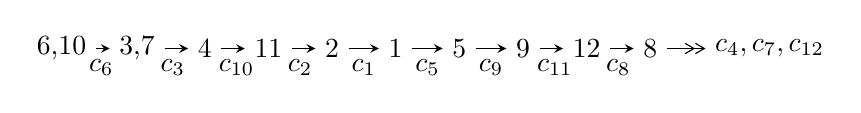
\begin{tikzpicture}[x=23pt, y=7pt]
	% node
	\node (A0) at (-1/8, 0) {6,10};
	\node (A1) at (17/16, 0) {3,7};
	\node (A2) at (17/8, 0) {4};
	\node (A3) at (25/8, 0) {11};
	\node (A4) at (33/8, 0) {2};
	\node (A5) at (41/8, 0) {1};
	\node (A6) at (49/8, 0) {5};
	\node (A7) at (57/8, 0) {9};
	\node (A8) at (65/8, 0) {12};
	\node (A9) at (73/8, 0) {8};
	\node (C1) at (1/2, -1) {$c_{6}$};
	\node (C2) at (13/8, -1) {$c_{3}$};
	\node (C3) at (21/8, -1) {$c_{10}$};
	\node (C4) at (29/8, -1) {$c_{2}$};
	\node (C5) at (37/8, -1) {$c_{1}$};
	\node (C6) at (45/8, -1) {$c_{5}$};
	\node (C7) at (53/8, -1) {$c_{9}$};
	\node (C8) at (61/8, -1) {$c_{11}$};
	\node (C9) at (69/8, -1) {$c_{8}$};
	\node (A10) at (11, 0) {$c_{4},c_{7},c_{12}$};

	% edge
	\draw[->,>=stealth]	
	(A0) edge (A1) (A1) edge (A2) (A2) edge (A3) (A3) edge (A4) (A4) edge (A5) (A5) edge (A6) (A6) edge (A7) (A7) edge (A8) (A8) edge (A9) ;
	\draw[->>,>={angle 60}]	
	(A9) edge (A10);
\end{tikzpicture} \\ 

\end{tabular} \\

\footnotetext{
The image of knot diagram is generated by the software ``\textbf{Draw programme}" developed by Andrew Bartholomew(\url{http://www.layer8.co.uk/maths/draw/index.htm\#Running-draw}), where we modified some parts for our purpose(\url{https://github.com/CATsTAILs/LinksPainter}).
}\phantom \\ \newline 
\centering \textbf{Ideals for irreducible components\footnotemark of $X_{\text{par}}$} 
 
\begin{align*}
I^u_{1}&=\langle 
-2.09914\times10^{1018} u^{144}-2.88524\times10^{1018} u^{143}+\cdots+3.72547\times10^{1017} b-1.57837\times10^{1020},\\
\phantom{I^u_{1}}&\phantom{= \langle  }-5.40470\times10^{1019} u^{144}-6.78220\times10^{1019} u^{143}+\cdots+1.15490\times10^{1019} a-6.04250\times10^{1021},\\
\phantom{I^u_{1}}&\phantom{= \langle  }u^{145}+u^{144}+\cdots+238 u-31\rangle \\
I^u_{2}&=\langle 
3.61659\times10^{28} u^{31}+7.73832\times10^{28} u^{30}+\cdots+3.44067\times10^{28} b-8.89248\times10^{28},\\
\phantom{I^u_{2}}&\phantom{= \langle  }5.39323\times10^{28} u^{31}+9.21403\times10^{28} u^{30}+\cdots+3.44067\times10^{28} a+1.58031\times10^{28},\;u^{32}+2 u^{31}+\cdots- u+1\rangle \\
\\
\end{align*}
\raggedright * 2 irreducible components of $\dim_{\mathbb{C}}=0$, with total 177 representations.\\
\footnotetext{All coefficients of polynomials are rational numbers. But the coefficients are sometimes approximated in decimal forms when there is not enough margin.}
\newpage
\renewcommand{\arraystretch}{1}
\centering \section*{I. $I^u_{1}= \langle -2.10\times10^{1018} u^{144}-2.89\times10^{1018} u^{143}+\cdots+3.73\times10^{1017} b-1.58\times10^{1020},\;-5.40\times10^{1019} u^{144}-6.78\times10^{1019} u^{143}+\cdots+1.15\times10^{1019} a-6.04\times10^{1021},\;u^{145}+u^{144}+\cdots+238 u-31 \rangle$}
\flushleft \textbf{(i) Arc colorings}\\
\begin{tabular}{m{7pt} m{180pt} m{7pt} m{180pt} }
\flushright $a_{6}=$&$\begin{pmatrix}1\\0\end{pmatrix}$ \\
\flushright $a_{10}=$&$\begin{pmatrix}0\\u\end{pmatrix}$ \\
\flushright $a_{3}=$&$\begin{pmatrix}4.67981 u^{144}+5.87256 u^{143}+\cdots-2318.63 u+523.207\\5.63455 u^{144}+7.74462 u^{143}+\cdots-2112.83 u+423.668\end{pmatrix}$ \\
\flushright $a_{7}=$&$\begin{pmatrix}1\\u^2\end{pmatrix}$ \\
\flushright $a_{4}=$&$\begin{pmatrix}-0.771919 u^{144}-1.57602 u^{143}+\cdots-344.597 u+136.514\\4.76589 u^{144}+6.61597 u^{143}+\cdots-1806.59 u+361.766\end{pmatrix}$ \\
\flushright $a_{11}=$&$\begin{pmatrix}2.79017 u^{144}+2.81371 u^{143}+\cdots-749.380 u+174.315\\-4.73297 u^{144}-6.56048 u^{143}+\cdots+2011.61 u-424.449\end{pmatrix}$ \\
\flushright $a_{2}=$&$\begin{pmatrix}-0.954736 u^{144}-1.87207 u^{143}+\cdots-205.798 u+99.5386\\5.63455 u^{144}+7.74462 u^{143}+\cdots-2112.83 u+423.668\end{pmatrix}$ \\
\flushright $a_{1}=$&$\begin{pmatrix}-1.31802 u^{144}-2.68164 u^{143}+\cdots+272.155 u-87.1026\\3.05808 u^{144}+3.78139 u^{143}+\cdots-1380.60 u+310.975\end{pmatrix}$ \\
\flushright $a_{5}=$&$\begin{pmatrix}3.84388 u^{144}+6.25083 u^{143}+\cdots-1397.32 u+245.504\\3.38549 u^{144}+4.43042 u^{143}+\cdots-1403.13 u+273.429\end{pmatrix}$ \\
\flushright $a_{9}=$&$\begin{pmatrix}6.45647 u^{144}+8.13085 u^{143}+\cdots-2347.32 u+522.309\\1.06667 u^{144}+1.24334 u^{143}+\cdots-411.667 u+76.4553\end{pmatrix}$ \\
\flushright $a_{12}=$&$\begin{pmatrix}7.52566 u^{144}+9.42017 u^{143}+\cdots-3397.01 u+725.029\\-7.30654 u^{144}-9.43795 u^{143}+\cdots+3301.93 u-734.941\end{pmatrix}$ \\
\flushright $a_{8}=$&$\begin{pmatrix}1.58406 u^{144}+3.01115 u^{143}+\cdots+35.0302 u-71.9586\\-2.19792 u^{144}-2.14369 u^{143}+\cdots+1374.66 u-309.390\end{pmatrix}$\\&\end{tabular}
\flushleft \textbf{(ii) Obstruction class $= -1$}\\~\\
\flushleft \textbf{(iii) Cusp Shapes $= 5.57129 u^{144}+6.71330 u^{143}+\cdots-3177.35 u+441.593$}\\~\\
\newpage\renewcommand{\arraystretch}{1}
\flushleft \textbf{(iv) u-Polynomials at the component}\newline \\
\begin{tabular}{m{50pt}|m{274pt}}
Crossings & \hspace{64pt}u-Polynomials at each crossing \\
\hline $$\begin{aligned}c_{1},c_{4}\end{aligned}$$&$\begin{aligned}
&u^{145}+6 u^{144}+\cdots+241016 u+53041
\end{aligned}$\\
\hline $$\begin{aligned}c_{2}\end{aligned}$$&$\begin{aligned}
&u^{145}-8 u^{144}+\cdots+31 u+1
\end{aligned}$\\
\hline $$\begin{aligned}c_{3}\end{aligned}$$&$\begin{aligned}
&u^{145}-25 u^{143}+\cdots-366697 u+53551
\end{aligned}$\\
\hline $$\begin{aligned}c_{5}\end{aligned}$$&$\begin{aligned}
&u^{145}-2 u^{144}+\cdots-584109 u+262673
\end{aligned}$\\
\hline $$\begin{aligned}c_{6}\end{aligned}$$&$\begin{aligned}
&u^{145}- u^{144}+\cdots+238 u+31
\end{aligned}$\\
\hline $$\begin{aligned}c_{7}\end{aligned}$$&$\begin{aligned}
&u^{145}+4 u^{144}+\cdots+220494628 u+11977767
\end{aligned}$\\
\hline $$\begin{aligned}c_{8},c_{11},c_{12}\end{aligned}$$&$\begin{aligned}
&u^{145}+6 u^{144}+\cdots-13 u+1
\end{aligned}$\\
\hline $$\begin{aligned}c_{9}\end{aligned}$$&$\begin{aligned}
&u^{145}-10 u^{143}+\cdots-2690 u+1025
\end{aligned}$\\
\hline $$\begin{aligned}c_{10}\end{aligned}$$&$\begin{aligned}
&u^{145}+4 u^{144}+\cdots-193 u+27
\end{aligned}$\\
\hline
\end{tabular}\\~\\
\newpage\renewcommand{\arraystretch}{1}
\flushleft \textbf{(v) Riley Polynomials at the component}\newline \\
\begin{tabular}{m{50pt}|m{274pt}}
Crossings & \hspace{64pt}Riley Polynomials at each crossing \\
\hline $$\begin{aligned}c_{1},c_{4}\end{aligned}$$&$\begin{aligned}
&y^{145}+114 y^{144}+\cdots-109382835062 y-2813347681
\end{aligned}$\\
\hline $$\begin{aligned}c_{2}\end{aligned}$$&$\begin{aligned}
&y^{145}+8 y^{144}+\cdots+245 y-1
\end{aligned}$\\
\hline $$\begin{aligned}c_{3}\end{aligned}$$&$\begin{aligned}
&y^{145}-50 y^{144}+\cdots+55811088111 y-2867709601
\end{aligned}$\\
\hline $$\begin{aligned}c_{5}\end{aligned}$$&$\begin{aligned}
&y^{145}+48 y^{144}+\cdots-7065213404445 y-68997104929
\end{aligned}$\\
\hline $$\begin{aligned}c_{6}\end{aligned}$$&$\begin{aligned}
&y^{145}-17 y^{144}+\cdots+83242 y-961
\end{aligned}$\\
\hline $$\begin{aligned}c_{7}\end{aligned}$$&$\begin{aligned}
&y^{145}+38 y^{144}+\cdots-9969062284337030 y-143466902306289
\end{aligned}$\\
\hline $$\begin{aligned}c_{8},c_{11},c_{12}\end{aligned}$$&$\begin{aligned}
&y^{145}+148 y^{144}+\cdots-23 y-1
\end{aligned}$\\
\hline $$\begin{aligned}c_{9}\end{aligned}$$&$\begin{aligned}
&y^{145}-20 y^{144}+\cdots-85056950 y-1050625
\end{aligned}$\\
\hline $$\begin{aligned}c_{10}\end{aligned}$$&$\begin{aligned}
&y^{145}+32 y^{144}+\cdots-44723 y-729
\end{aligned}$\\
\hline
\end{tabular}\\~\\
\newpage\flushleft \textbf{(vi) Complex Volumes and Cusp Shapes}
$$\begin{array}{c|c|c}  
\text{Solutions to }I^u_{1}& \I (\text{vol} + \sqrt{-1}CS) & \text{Cusp shape}\\
 \hline 
\begin{aligned}
u &= -0.175233 + 0.993312 I \\
a &= -1.50509 + 0.99291 I \\
b &= \phantom{-}0.984730 + 0.148375 I\end{aligned}
 & \phantom{-}9.85859 + 8.66525 I & \phantom{-0.000000 } 0 \\ \hline\begin{aligned}
u &= -0.175233 - 0.993312 I \\
a &= -1.50509 - 0.99291 I \\
b &= \phantom{-}0.984730 - 0.148375 I\end{aligned}
 & \phantom{-}9.85859 - 8.66525 I & \phantom{-0.000000 } 0 \\ \hline\begin{aligned}
u &= -0.270642 + 0.973406 I \\
a &= \phantom{-}0.37280 - 1.37338 I \\
b &= -0.197005 + 0.309824 I\end{aligned}
 & \phantom{-}8.44939 + 3.42419 I & \phantom{-0.000000 } 0 \\ \hline\begin{aligned}
u &= -0.270642 - 0.973406 I \\
a &= \phantom{-}0.37280 + 1.37338 I \\
b &= -0.197005 - 0.309824 I\end{aligned}
 & \phantom{-}8.44939 - 3.42419 I & \phantom{-0.000000 } 0 \\ \hline\begin{aligned}
u &= -0.457505 + 0.873801 I \\
a &= \phantom{-}0.001931 - 1.056370 I \\
b &= -1.10167 - 1.39405 I\end{aligned}
 & \phantom{-}10.5547 + 10.4208 I & \phantom{-0.000000 } 0 \\ \hline\begin{aligned}
u &= -0.457505 - 0.873801 I \\
a &= \phantom{-}0.001931 + 1.056370 I \\
b &= -1.10167 + 1.39405 I\end{aligned}
 & \phantom{-}10.5547 - 10.4208 I & \phantom{-0.000000 } 0 \\ \hline\begin{aligned}
u &= \phantom{-}0.853690 + 0.554488 I \\
a &= \phantom{-}0.24679 - 1.57189 I \\
b &= \phantom{-}1.20444 - 1.27727 I\end{aligned}
 & \phantom{-}6.99182 - 4.73153 I & \phantom{-0.000000 } 0 \\ \hline\begin{aligned}
u &= \phantom{-}0.853690 - 0.554488 I \\
a &= \phantom{-}0.24679 + 1.57189 I \\
b &= \phantom{-}1.20444 + 1.27727 I\end{aligned}
 & \phantom{-}6.99182 + 4.73153 I & \phantom{-0.000000 } 0 \\ \hline\begin{aligned}
u &= -0.779856 + 0.578252 I \\
a &= \phantom{-}0.08031 + 1.59012 I \\
b &= \phantom{-}0.95266 + 1.16365 I\end{aligned}
 & \phantom{-}1.26897 + 4.48898 I & \phantom{-0.000000 } 0 \\ \hline\begin{aligned}
u &= -0.779856 - 0.578252 I \\
a &= \phantom{-}0.08031 - 1.59012 I \\
b &= \phantom{-}0.95266 - 1.16365 I\end{aligned}
 & \phantom{-}1.26897 - 4.48898 I & \phantom{-0.000000 } 0\\
 \hline 
 \end{array}$$\newpage$$\begin{array}{c|c|c}  
\text{Solutions to }I^u_{1}& \I (\text{vol} + \sqrt{-1}CS) & \text{Cusp shape}\\
 \hline 
\begin{aligned}
u &= \phantom{-}0.966669\phantom{ +0.000000I} \\
a &= \phantom{-}0.511382\phantom{ +0.000000I} \\
b &= -0.230935\phantom{ +0.000000I}\end{aligned}
 & -1.29626\phantom{ +0.000000I} & \phantom{-0.000000 } 0 \\ \hline\begin{aligned}
u &= -0.842836 + 0.473333 I \\
a &= \phantom{-}0.114165 + 0.731850 I \\
b &= \phantom{-}1.34113 + 1.21796 I\end{aligned}
 & \phantom{-}3.56283 + 6.56801 I & \phantom{-0.000000 } 0 \\ \hline\begin{aligned}
u &= -0.842836 - 0.473333 I \\
a &= \phantom{-}0.114165 - 0.731850 I \\
b &= \phantom{-}1.34113 - 1.21796 I\end{aligned}
 & \phantom{-}3.56283 - 6.56801 I & \phantom{-0.000000 } 0 \\ \hline\begin{aligned}
u &= \phantom{-}0.328978 + 0.898582 I \\
a &= \phantom{-}0.249788 + 1.287120 I \\
b &= -0.0809638 - 0.0060685 I\end{aligned}
 & \phantom{-}2.99294 - 2.90031 I & \phantom{-0.000000 } 0 \\ \hline\begin{aligned}
u &= \phantom{-}0.328978 - 0.898582 I \\
a &= \phantom{-}0.249788 - 1.287120 I \\
b &= -0.0809638 + 0.0060685 I\end{aligned}
 & \phantom{-}2.99294 + 2.90031 I & \phantom{-0.000000 } 0 \\ \hline\begin{aligned}
u &= \phantom{-}0.985932 + 0.403210 I \\
a &= \phantom{-}0.773146 - 0.957633 I \\
b &= \phantom{-}1.131940 - 0.532852 I\end{aligned}
 & \phantom{-}7.33618 - 2.02582 I & \phantom{-0.000000 } 0 \\ \hline\begin{aligned}
u &= \phantom{-}0.985932 - 0.403210 I \\
a &= \phantom{-}0.773146 + 0.957633 I \\
b &= \phantom{-}1.131940 + 0.532852 I\end{aligned}
 & \phantom{-}7.33618 + 2.02582 I & \phantom{-0.000000 } 0 \\ \hline\begin{aligned}
u &= -0.927787 + 0.062557 I \\
a &= \phantom{-}0.364733 + 0.697991 I \\
b &= \phantom{-}0.529992 + 1.300080 I\end{aligned}
 & \phantom{-}0.88219 + 1.22730 I & \phantom{-0.000000 } 0 \\ \hline\begin{aligned}
u &= -0.927787 - 0.062557 I \\
a &= \phantom{-}0.364733 - 0.697991 I \\
b &= \phantom{-}0.529992 - 1.300080 I\end{aligned}
 & \phantom{-}0.88219 - 1.22730 I & \phantom{-0.000000 } 0 \\ \hline\begin{aligned}
u &= \phantom{-}0.794588 + 0.464628 I \\
a &= \phantom{-}0.851818 + 0.312631 I \\
b &= -0.096564 + 0.431521 I\end{aligned}
 & -1.38971 - 0.42921 I & \phantom{-0.000000 } 0\\
 \hline 
 \end{array}$$\newpage$$\begin{array}{c|c|c}  
\text{Solutions to }I^u_{1}& \I (\text{vol} + \sqrt{-1}CS) & \text{Cusp shape}\\
 \hline 
\begin{aligned}
u &= \phantom{-}0.794588 - 0.464628 I \\
a &= \phantom{-}0.851818 - 0.312631 I \\
b &= -0.096564 - 0.431521 I\end{aligned}
 & -1.38971 + 0.42921 I & \phantom{-0.000000 } 0 \\ \hline\begin{aligned}
u &= \phantom{-}0.809274 + 0.438011 I \\
a &= -0.245927 - 0.502995 I \\
b &= -0.894106 - 0.707102 I\end{aligned}
 & -2.09607 - 0.26844 I & \phantom{-0.000000 } 0 \\ \hline\begin{aligned}
u &= \phantom{-}0.809274 - 0.438011 I \\
a &= -0.245927 + 0.502995 I \\
b &= -0.894106 + 0.707102 I\end{aligned}
 & -2.09607 + 0.26844 I & \phantom{-0.000000 } 0 \\ \hline\begin{aligned}
u &= \phantom{-}0.834733 + 0.378244 I \\
a &= \phantom{-}0.120339 - 0.828214 I \\
b &= \phantom{-}1.04293 - 1.22525 I\end{aligned}
 & -1.62770 - 3.91436 I & \phantom{-0.000000 } 0 \\ \hline\begin{aligned}
u &= \phantom{-}0.834733 - 0.378244 I \\
a &= \phantom{-}0.120339 + 0.828214 I \\
b &= \phantom{-}1.04293 + 1.22525 I\end{aligned}
 & -1.62770 + 3.91436 I & \phantom{-0.000000 } 0 \\ \hline\begin{aligned}
u &= \phantom{-}0.432543 + 0.996527 I \\
a &= \phantom{-}0.027076 + 1.027480 I \\
b &= -0.76676 + 1.24530 I\end{aligned}
 & \phantom{-}4.17885 - 5.54834 I & \phantom{-0.000000 } 0 \\ \hline\begin{aligned}
u &= \phantom{-}0.432543 - 0.996527 I \\
a &= \phantom{-}0.027076 - 1.027480 I \\
b &= -0.76676 - 1.24530 I\end{aligned}
 & \phantom{-}4.17885 + 5.54834 I & \phantom{-0.000000 } 0 \\ \hline\begin{aligned}
u &= -1.066270 + 0.247929 I \\
a &= -0.206778 + 0.289540 I \\
b &= -1.200350 + 0.617183 I\end{aligned}
 & \phantom{-}3.12685 - 0.12674 I & \phantom{-0.000000 } 0 \\ \hline\begin{aligned}
u &= -1.066270 - 0.247929 I \\
a &= -0.206778 - 0.289540 I \\
b &= -1.200350 - 0.617183 I\end{aligned}
 & \phantom{-}3.12685 + 0.12674 I & \phantom{-0.000000 } 0 \\ \hline\begin{aligned}
u &= -0.162959 + 1.082590 I \\
a &= \phantom{-}0.198535 - 0.111941 I \\
b &= \phantom{-}0.648377 - 0.887697 I\end{aligned}
 & \phantom{-}2.09440 - 1.76971 I & \phantom{-0.000000 } 0\\
 \hline 
 \end{array}$$\newpage$$\begin{array}{c|c|c}  
\text{Solutions to }I^u_{1}& \I (\text{vol} + \sqrt{-1}CS) & \text{Cusp shape}\\
 \hline 
\begin{aligned}
u &= -0.162959 - 1.082590 I \\
a &= \phantom{-}0.198535 + 0.111941 I \\
b &= \phantom{-}0.648377 + 0.887697 I\end{aligned}
 & \phantom{-}2.09440 + 1.76971 I & \phantom{-0.000000 } 0 \\ \hline\begin{aligned}
u &= -0.967028 + 0.516281 I \\
a &= \phantom{-}1.004840 + 0.297297 I \\
b &= \phantom{-}0.219267 - 0.422014 I\end{aligned}
 & \phantom{-}3.49440 - 1.89700 I & \phantom{-0.000000 } 0 \\ \hline\begin{aligned}
u &= -0.967028 - 0.516281 I \\
a &= \phantom{-}1.004840 - 0.297297 I \\
b &= \phantom{-}0.219267 + 0.422014 I\end{aligned}
 & \phantom{-}3.49440 + 1.89700 I & \phantom{-0.000000 } 0 \\ \hline\begin{aligned}
u &= \phantom{-}1.101490 + 0.040866 I \\
a &= \phantom{-}0.48056 - 1.45999 I \\
b &= \phantom{-}0.024912 - 0.558133 I\end{aligned}
 & -0.861624 + 0.409948 I & \phantom{-0.000000 } 0 \\ \hline\begin{aligned}
u &= \phantom{-}1.101490 - 0.040866 I \\
a &= \phantom{-}0.48056 + 1.45999 I \\
b &= \phantom{-}0.024912 + 0.558133 I\end{aligned}
 & -0.861624 - 0.409948 I & \phantom{-0.000000 } 0 \\ \hline\begin{aligned}
u &= -0.722310 + 0.843040 I \\
a &= \phantom{-}0.34411 - 1.42106 I \\
b &= -0.763936 - 0.462647 I\end{aligned}
 & \phantom{-}5.23556 + 5.23001 I & \phantom{-0.000000 } 0 \\ \hline\begin{aligned}
u &= -0.722310 - 0.843040 I \\
a &= \phantom{-}0.34411 + 1.42106 I \\
b &= -0.763936 + 0.462647 I\end{aligned}
 & \phantom{-}5.23556 - 5.23001 I & \phantom{-0.000000 } 0 \\ \hline\begin{aligned}
u &= \phantom{-}0.355968 + 0.798221 I \\
a &= -1.17073 - 1.66706 I \\
b &= \phantom{-}0.807566 - 0.466961 I\end{aligned}
 & \phantom{-}2.77202 - 6.23642 I & \phantom{-0.000000 } 0 \\ \hline\begin{aligned}
u &= \phantom{-}0.355968 - 0.798221 I \\
a &= -1.17073 + 1.66706 I \\
b &= \phantom{-}0.807566 + 0.466961 I\end{aligned}
 & \phantom{-}2.77202 + 6.23642 I & \phantom{-0.000000 } 0 \\ \hline\begin{aligned}
u &= -0.711648 + 0.877783 I \\
a &= \phantom{-}0.045504 - 1.080010 I \\
b &= -0.077228 - 1.046060 I\end{aligned}
 & \phantom{-}6.84476 + 0.58245 I & \phantom{-0.000000 } 0\\
 \hline 
 \end{array}$$\newpage$$\begin{array}{c|c|c}  
\text{Solutions to }I^u_{1}& \I (\text{vol} + \sqrt{-1}CS) & \text{Cusp shape}\\
 \hline 
\begin{aligned}
u &= -0.711648 - 0.877783 I \\
a &= \phantom{-}0.045504 + 1.080010 I \\
b &= -0.077228 + 1.046060 I\end{aligned}
 & \phantom{-}6.84476 - 0.58245 I & \phantom{-0.000000 } 0 \\ \hline\begin{aligned}
u &= -0.509051 + 1.017630 I \\
a &= \phantom{-}0.064952 - 0.952618 I \\
b &= -0.772460 - 0.661107 I\end{aligned}
 & \phantom{-}5.89302 + 0.19949 I & \phantom{-0.000000 } 0 \\ \hline\begin{aligned}
u &= -0.509051 - 1.017630 I \\
a &= \phantom{-}0.064952 + 0.952618 I \\
b &= -0.772460 + 0.661107 I\end{aligned}
 & \phantom{-}5.89302 - 0.19949 I & \phantom{-0.000000 } 0 \\ \hline\begin{aligned}
u &= \phantom{-}0.750068 + 0.374115 I \\
a &= \phantom{-}0.27446 - 1.75411 I \\
b &= \phantom{-}0.48114 - 1.55804 I\end{aligned}
 & \phantom{-}5.33434 - 5.39101 I & \phantom{-0.000000 } 0 \\ \hline\begin{aligned}
u &= \phantom{-}0.750068 - 0.374115 I \\
a &= \phantom{-}0.27446 + 1.75411 I \\
b &= \phantom{-}0.48114 + 1.55804 I\end{aligned}
 & \phantom{-}5.33434 + 5.39101 I & \phantom{-0.000000 } 0 \\ \hline\begin{aligned}
u &= \phantom{-}0.559310 + 1.043510 I \\
a &= -0.022095 + 0.894625 I \\
b &= -1.110140 + 0.547552 I\end{aligned}
 & \phantom{-}13.46280 + 2.57020 I & \phantom{-0.000000 } 0 \\ \hline\begin{aligned}
u &= \phantom{-}0.559310 - 1.043510 I \\
a &= -0.022095 - 0.894625 I \\
b &= -1.110140 - 0.547552 I\end{aligned}
 & \phantom{-}13.46280 - 2.57020 I & \phantom{-0.000000 } 0 \\ \hline\begin{aligned}
u &= \phantom{-}0.677087 + 0.322793 I \\
a &= \phantom{-}0.092962 + 0.965597 I \\
b &= \phantom{-}1.28360 + 1.51766 I\end{aligned}
 & \phantom{-}6.87184 - 10.70990 I & \phantom{-0.000000 } 0 \\ \hline\begin{aligned}
u &= \phantom{-}0.677087 - 0.322793 I \\
a &= \phantom{-}0.092962 - 0.965597 I \\
b &= \phantom{-}1.28360 - 1.51766 I\end{aligned}
 & \phantom{-}6.87184 + 10.70990 I & \phantom{-0.000000 } 0 \\ \hline\begin{aligned}
u &= -0.568846 + 1.113300 I \\
a &= \phantom{-}0.162339 + 0.183610 I \\
b &= \phantom{-}1.100390 + 0.403905 I\end{aligned}
 & \phantom{-}10.38580 + 4.15509 I & \phantom{-0.000000 } 0\\
 \hline 
 \end{array}$$\newpage$$\begin{array}{c|c|c}  
\text{Solutions to }I^u_{1}& \I (\text{vol} + \sqrt{-1}CS) & \text{Cusp shape}\\
 \hline 
\begin{aligned}
u &= -0.568846 - 1.113300 I \\
a &= \phantom{-}0.162339 - 0.183610 I \\
b &= \phantom{-}1.100390 - 0.403905 I\end{aligned}
 & \phantom{-}10.38580 - 4.15509 I & \phantom{-0.000000 } 0 \\ \hline\begin{aligned}
u &= -0.659678 + 1.064510 I \\
a &= \phantom{-}0.590704 - 0.199088 I \\
b &= -0.466431 - 0.492976 I\end{aligned}
 & \phantom{-}3.38993 + 3.85851 I & \phantom{-0.000000 } 0 \\ \hline\begin{aligned}
u &= -0.659678 - 1.064510 I \\
a &= \phantom{-}0.590704 + 0.199088 I \\
b &= -0.466431 + 0.492976 I\end{aligned}
 & \phantom{-}3.38993 - 3.85851 I & \phantom{-0.000000 } 0 \\ \hline\begin{aligned}
u &= -0.856740 + 0.927176 I \\
a &= -0.831698 + 0.861803 I \\
b &= \phantom{-}0.289995 + 0.586627 I\end{aligned}
 & \phantom{-}6.56094 + 5.30740 I & \phantom{-0.000000 } 0 \\ \hline\begin{aligned}
u &= -0.856740 - 0.927176 I \\
a &= -0.831698 - 0.861803 I \\
b &= \phantom{-}0.289995 - 0.586627 I\end{aligned}
 & \phantom{-}6.56094 - 5.30740 I & \phantom{-0.000000 } 0 \\ \hline\begin{aligned}
u &= \phantom{-}0.637639 + 0.329081 I \\
a &= -0.47670 + 2.53347 I \\
b &= -0.312601 + 0.534758 I\end{aligned}
 & -2.41986 - 3.05864 I & \phantom{-0.000000 } 0 \\ \hline\begin{aligned}
u &= \phantom{-}0.637639 - 0.329081 I \\
a &= -0.47670 - 2.53347 I \\
b &= -0.312601 - 0.534758 I\end{aligned}
 & -2.41986 + 3.05864 I & \phantom{-0.000000 } 0 \\ \hline\begin{aligned}
u &= -1.136110 + 0.646165 I \\
a &= -0.294255 + 0.471721 I \\
b &= -0.702647 + 1.194120 I\end{aligned}
 & \phantom{-}2.22638 - 0.12544 I & \phantom{-0.000000 } 0 \\ \hline\begin{aligned}
u &= -1.136110 - 0.646165 I \\
a &= -0.294255 - 0.471721 I \\
b &= -0.702647 - 1.194120 I\end{aligned}
 & \phantom{-}2.22638 + 0.12544 I & \phantom{-0.000000 } 0 \\ \hline\begin{aligned}
u &= -1.170270 + 0.605888 I \\
a &= \phantom{-}0.285001 + 0.717823 I \\
b &= \phantom{-}0.774449 + 0.730807 I\end{aligned}
 & \phantom{-}0.46547 + 2.09210 I & \phantom{-0.000000 } 0\\
 \hline 
 \end{array}$$\newpage$$\begin{array}{c|c|c}  
\text{Solutions to }I^u_{1}& \I (\text{vol} + \sqrt{-1}CS) & \text{Cusp shape}\\
 \hline 
\begin{aligned}
u &= -1.170270 - 0.605888 I \\
a &= \phantom{-}0.285001 - 0.717823 I \\
b &= \phantom{-}0.774449 - 0.730807 I\end{aligned}
 & \phantom{-}0.46547 - 2.09210 I & \phantom{-0.000000 } 0 \\ \hline\begin{aligned}
u &= -0.104328 + 0.661044 I \\
a &= -0.03414 - 1.78053 I \\
b &= \phantom{-}0.620897 + 0.232105 I\end{aligned}
 & \phantom{-}8.37051 + 1.60856 I & \phantom{-0.000000 } 0 \\ \hline\begin{aligned}
u &= -0.104328 - 0.661044 I \\
a &= -0.03414 + 1.78053 I \\
b &= \phantom{-}0.620897 - 0.232105 I\end{aligned}
 & \phantom{-}8.37051 - 1.60856 I & \phantom{-0.000000 } 0 \\ \hline\begin{aligned}
u &= \phantom{-}0.661436 + 0.014358 I \\
a &= \phantom{-}0.173534 - 1.294400 I \\
b &= -0.95347 - 1.62284 I\end{aligned}
 & \phantom{-}1.32185 - 4.06716 I & \phantom{-0.000000 } 0 \\ \hline\begin{aligned}
u &= \phantom{-}0.661436 - 0.014358 I \\
a &= \phantom{-}0.173534 + 1.294400 I \\
b &= -0.95347 + 1.62284 I\end{aligned}
 & \phantom{-}1.32185 + 4.06716 I & \phantom{-0.000000 } 0 \\ \hline\begin{aligned}
u &= -0.578994 + 0.298296 I \\
a &= -0.71154 + 1.53149 I \\
b &= \phantom{-}0.929249 + 0.898528 I\end{aligned}
 & \phantom{-}0.07179 + 3.70060 I & \phantom{-0.000000 } 0 \\ \hline\begin{aligned}
u &= -0.578994 - 0.298296 I \\
a &= -0.71154 - 1.53149 I \\
b &= \phantom{-}0.929249 - 0.898528 I\end{aligned}
 & \phantom{-}0.07179 - 3.70060 I & \phantom{-0.000000 } 0 \\ \hline\begin{aligned}
u &= -0.550613 + 0.347580 I \\
a &= \phantom{-}0.038949 - 0.919566 I \\
b &= \phantom{-}1.45706 - 1.12848 I\end{aligned}
 & \phantom{-}0.68944 + 6.98932 I & \phantom{-0.000000 } 0 \\ \hline\begin{aligned}
u &= -0.550613 - 0.347580 I \\
a &= \phantom{-}0.038949 + 0.919566 I \\
b &= \phantom{-}1.45706 + 1.12848 I\end{aligned}
 & \phantom{-}0.68944 - 6.98932 I & \phantom{-0.000000 } 0 \\ \hline\begin{aligned}
u &= -0.613680 + 0.203109 I \\
a &= \phantom{-}2.84986 - 1.48270 I \\
b &= -0.155422 - 0.487057 I\end{aligned}
 & \phantom{-}0.30339 + 6.35289 I & \phantom{-0.000000 } 0. - 25.1026 I\\
 \hline 
 \end{array}$$\newpage$$\begin{array}{c|c|c}  
\text{Solutions to }I^u_{1}& \I (\text{vol} + \sqrt{-1}CS) & \text{Cusp shape}\\
 \hline 
\begin{aligned}
u &= -0.613680 - 0.203109 I \\
a &= \phantom{-}2.84986 + 1.48270 I \\
b &= -0.155422 + 0.487057 I\end{aligned}
 & \phantom{-}0.30339 - 6.35289 I & \phantom{-0.000000 -}0. + 25.1026 I \\ \hline\begin{aligned}
u &= \phantom{-}0.591375 + 0.256999 I \\
a &= -0.55267 - 2.24509 I \\
b &= \phantom{-}0.980139 - 1.004110 I\end{aligned}
 & \phantom{-}5.89423 - 4.66757 I & \phantom{-0.000000 } 0 \\ \hline\begin{aligned}
u &= \phantom{-}0.591375 - 0.256999 I \\
a &= -0.55267 + 2.24509 I \\
b &= \phantom{-}0.980139 + 1.004110 I\end{aligned}
 & \phantom{-}5.89423 + 4.66757 I & \phantom{-0.000000 } 0 \\ \hline\begin{aligned}
u &= \phantom{-}1.072280 + 0.838787 I \\
a &= -0.073824 - 0.857507 I \\
b &= \phantom{-}0.98899 - 1.14772 I\end{aligned}
 & -1.91092 - 4.53651 I & \phantom{-0.000000 } 0 \\ \hline\begin{aligned}
u &= \phantom{-}1.072280 - 0.838787 I \\
a &= -0.073824 + 0.857507 I \\
b &= \phantom{-}0.98899 + 1.14772 I\end{aligned}
 & -1.91092 + 4.53651 I & \phantom{-0.000000 } 0 \\ \hline\begin{aligned}
u &= -0.625242 + 0.104972 I \\
a &= \phantom{-}0.810423 + 0.997280 I \\
b &= \phantom{-}0.556069 + 0.687308 I\end{aligned}
 & \phantom{-}0.68161 + 1.58841 I & \phantom{-0.000000 } 0 \\ \hline\begin{aligned}
u &= -0.625242 - 0.104972 I \\
a &= \phantom{-}0.810423 - 0.997280 I \\
b &= \phantom{-}0.556069 - 0.687308 I\end{aligned}
 & \phantom{-}0.68161 - 1.58841 I & \phantom{-0.000000 } 0 \\ \hline\begin{aligned}
u &= \phantom{-}0.562625 + 0.271590 I \\
a &= \phantom{-}0.98707 - 1.67557 I \\
b &= \phantom{-}0.995209 - 0.465961 I\end{aligned}
 & \phantom{-}7.40415 - 1.90436 I & \phantom{-0.000000 } 0 \\ \hline\begin{aligned}
u &= \phantom{-}0.562625 - 0.271590 I \\
a &= \phantom{-}0.98707 + 1.67557 I \\
b &= \phantom{-}0.995209 + 0.465961 I\end{aligned}
 & \phantom{-}7.40415 + 1.90436 I & \phantom{-0.000000 } 0 \\ \hline\begin{aligned}
u &= \phantom{-}0.369904 + 0.468983 I \\
a &= -0.603481 + 0.212699 I \\
b &= \phantom{-}1.183390 - 0.469764 I\end{aligned}
 & \phantom{-}1.58948 - 2.62456 I & \phantom{-0.000000 -}0. + 3.62743 I\\
 \hline 
 \end{array}$$\newpage$$\begin{array}{c|c|c}  
\text{Solutions to }I^u_{1}& \I (\text{vol} + \sqrt{-1}CS) & \text{Cusp shape}\\
 \hline 
\begin{aligned}
u &= \phantom{-}0.369904 - 0.468983 I \\
a &= -0.603481 - 0.212699 I \\
b &= \phantom{-}1.183390 + 0.469764 I\end{aligned}
 & \phantom{-}1.58948 + 2.62456 I & \phantom{-0.000000 } 0. - 3.62743 I \\ \hline\begin{aligned}
u &= \phantom{-}0.371064 + 0.461167 I \\
a &= -0.268667 + 0.858423 I \\
b &= \phantom{-}1.251690 + 0.170593 I\end{aligned}
 & \phantom{-}1.70497 - 2.66262 I & \phantom{-0.000000 -}0. + 6.62401 I \\ \hline\begin{aligned}
u &= \phantom{-}0.371064 - 0.461167 I \\
a &= -0.268667 - 0.858423 I \\
b &= \phantom{-}1.251690 - 0.170593 I\end{aligned}
 & \phantom{-}1.70497 + 2.66262 I & \phantom{-0.000000 } 0. - 6.62401 I \\ \hline\begin{aligned}
u &= \phantom{-}1.083310 + 0.908174 I \\
a &= \phantom{-}0.016723 + 1.094320 I \\
b &= -0.831442 + 1.025920 I\end{aligned}
 & -3.19557 - 5.94519 I & \phantom{-0.000000 } 0 \\ \hline\begin{aligned}
u &= \phantom{-}1.083310 - 0.908174 I \\
a &= \phantom{-}0.016723 - 1.094320 I \\
b &= -0.831442 - 1.025920 I\end{aligned}
 & -3.19557 + 5.94519 I & \phantom{-0.000000 } 0 \\ \hline\begin{aligned}
u &= \phantom{-}0.497529 + 0.282324 I \\
a &= \phantom{-}3.82000 + 0.64029 I \\
b &= -0.313502 + 0.520244 I\end{aligned}
 & \phantom{-}7.70025 - 10.38410 I & -6.0000 + 16.0066 I \\ \hline\begin{aligned}
u &= \phantom{-}0.497529 - 0.282324 I \\
a &= \phantom{-}3.82000 - 0.64029 I \\
b &= -0.313502 - 0.520244 I\end{aligned}
 & \phantom{-}7.70025 + 10.38410 I & -6.0000 - 16.0066 I \\ \hline\begin{aligned}
u &= -0.486754 + 0.297305 I \\
a &= \phantom{-}0.88123 + 2.29211 I \\
b &= \phantom{-}0.006286 + 0.981261 I\end{aligned}
 & \phantom{-}0.46950 + 3.52931 I & -11.59746 - 5.64649 I \\ \hline\begin{aligned}
u &= -0.486754 - 0.297305 I \\
a &= \phantom{-}0.88123 - 2.29211 I \\
b &= \phantom{-}0.006286 - 0.981261 I\end{aligned}
 & \phantom{-}0.46950 - 3.52931 I & -11.59746 + 5.64649 I \\ \hline\begin{aligned}
u &= -1.00830 + 1.01817 I \\
a &= -0.266712 + 0.840438 I \\
b &= \phantom{-}1.23990 + 1.10914 I\end{aligned}
 & \phantom{-}2.55761 + 7.40596 I & \phantom{-0.000000 } 0\\
 \hline 
 \end{array}$$\newpage$$\begin{array}{c|c|c}  
\text{Solutions to }I^u_{1}& \I (\text{vol} + \sqrt{-1}CS) & \text{Cusp shape}\\
 \hline 
\begin{aligned}
u &= -1.00830 - 1.01817 I \\
a &= -0.266712 - 0.840438 I \\
b &= \phantom{-}1.23990 - 1.10914 I\end{aligned}
 & \phantom{-}2.55761 - 7.40596 I & \phantom{-0.000000 } 0 \\ \hline\begin{aligned}
u &= -1.18863 + 0.80119 I \\
a &= -0.047559 + 0.688065 I \\
b &= \phantom{-}0.486127 + 1.210110 I\end{aligned}
 & \phantom{-}1.08652 + 2.07918 I & \phantom{-0.000000 } 0 \\ \hline\begin{aligned}
u &= -1.18863 - 0.80119 I \\
a &= -0.047559 - 0.688065 I \\
b &= \phantom{-}0.486127 - 1.210110 I\end{aligned}
 & \phantom{-}1.08652 - 2.07918 I & \phantom{-0.000000 } 0 \\ \hline\begin{aligned}
u &= -0.556768 + 0.038672 I \\
a &= \phantom{-}0.031722 + 1.231130 I \\
b &= -1.22823 + 1.28194 I\end{aligned}
 & -3.65244 + 1.72670 I & -21.4514 - 5.0713 I \\ \hline\begin{aligned}
u &= -0.556768 - 0.038672 I \\
a &= \phantom{-}0.031722 - 1.231130 I \\
b &= -1.22823 - 1.28194 I\end{aligned}
 & -3.65244 - 1.72670 I & -21.4514 + 5.0713 I \\ \hline\begin{aligned}
u &= \phantom{-}1.08513 + 0.95150 I \\
a &= -0.170686 - 0.386102 I \\
b &= -0.233957 - 0.718289 I\end{aligned}
 & -2.26919 - 0.66351 I & \phantom{-0.000000 } 0 \\ \hline\begin{aligned}
u &= \phantom{-}1.08513 - 0.95150 I \\
a &= -0.170686 + 0.386102 I \\
b &= -0.233957 + 0.718289 I\end{aligned}
 & -2.26919 + 0.66351 I & \phantom{-0.000000 } 0 \\ \hline\begin{aligned}
u &= \phantom{-}0.529427 + 0.121719 I \\
a &= -2.50547 - 2.05101 I \\
b &= \phantom{-}0.294527 - 0.823997 I\end{aligned}
 & \phantom{-}1.89483 - 4.47916 I & -13.3702 + 6.6534 I \\ \hline\begin{aligned}
u &= \phantom{-}0.529427 - 0.121719 I \\
a &= -2.50547 + 2.05101 I \\
b &= \phantom{-}0.294527 + 0.823997 I\end{aligned}
 & \phantom{-}1.89483 + 4.47916 I & -13.3702 - 6.6534 I \\ \hline\begin{aligned}
u &= -1.13569 + 0.91956 I \\
a &= -0.041880 - 1.052690 I \\
b &= -1.00525 - 1.11497 I\end{aligned}
 & -4.11430 + 10.02680 I & \phantom{-0.000000 } 0\\
 \hline 
 \end{array}$$\newpage$$\begin{array}{c|c|c}  
\text{Solutions to }I^u_{1}& \I (\text{vol} + \sqrt{-1}CS) & \text{Cusp shape}\\
 \hline 
\begin{aligned}
u &= -1.13569 - 0.91956 I \\
a &= -0.041880 + 1.052690 I \\
b &= -1.00525 + 1.11497 I\end{aligned}
 & -4.11430 - 10.02680 I & \phantom{-0.000000 } 0 \\ \hline\begin{aligned}
u &= -0.514987 + 0.053999 I \\
a &= -2.24549 - 2.98451 I \\
b &= \phantom{-}0.017963 - 0.599980 I\end{aligned}
 & -3.51088 - 1.35231 I & -23.2910 + 3.3744 I \\ \hline\begin{aligned}
u &= -0.514987 - 0.053999 I \\
a &= -2.24549 + 2.98451 I \\
b &= \phantom{-}0.017963 + 0.599980 I\end{aligned}
 & -3.51088 + 1.35231 I & -23.2910 - 3.3744 I \\ \hline\begin{aligned}
u &= -1.46228 + 0.26379 I \\
a &= -0.482951 - 0.780205 I \\
b &= -0.420296 - 0.640012 I\end{aligned}
 & \phantom{-}6.42247 + 5.98655 I & \phantom{-0.000000 } 0 \\ \hline\begin{aligned}
u &= -1.46228 - 0.26379 I \\
a &= -0.482951 + 0.780205 I \\
b &= -0.420296 + 0.640012 I\end{aligned}
 & \phantom{-}6.42247 - 5.98655 I & \phantom{-0.000000 } 0 \\ \hline\begin{aligned}
u &= \phantom{-}1.17057 + 0.91668 I \\
a &= -0.101247 + 1.044950 I \\
b &= -1.14666 + 1.12493 I\end{aligned}
 & \phantom{-}1.95287 - 13.11790 I & \phantom{-0.000000 } 0 \\ \hline\begin{aligned}
u &= \phantom{-}1.17057 - 0.91668 I \\
a &= -0.101247 - 1.044950 I \\
b &= -1.14666 - 1.12493 I\end{aligned}
 & \phantom{-}1.95287 + 13.11790 I & \phantom{-0.000000 } 0 \\ \hline\begin{aligned}
u &= \phantom{-}1.06134 + 1.15983 I \\
a &= \phantom{-}0.290866 + 0.840933 I \\
b &= -1.08775 + 1.01185 I\end{aligned}
 & -1.48980 - 7.19259 I & \phantom{-0.000000 } 0 \\ \hline\begin{aligned}
u &= \phantom{-}1.06134 - 1.15983 I \\
a &= \phantom{-}0.290866 - 0.840933 I \\
b &= -1.08775 - 1.01185 I\end{aligned}
 & -1.48980 + 7.19259 I & \phantom{-0.000000 } 0 \\ \hline\begin{aligned}
u &= -1.00710 + 1.21075 I \\
a &= \phantom{-}0.396548 - 0.871295 I \\
b &= -1.23418 - 1.02046 I\end{aligned}
 & \phantom{-}3.78215 + 7.83286 I & \phantom{-0.000000 } 0\\
 \hline 
 \end{array}$$\newpage$$\begin{array}{c|c|c}  
\text{Solutions to }I^u_{1}& \I (\text{vol} + \sqrt{-1}CS) & \text{Cusp shape}\\
 \hline 
\begin{aligned}
u &= -1.00710 - 1.21075 I \\
a &= \phantom{-}0.396548 + 0.871295 I \\
b &= -1.23418 + 1.02046 I\end{aligned}
 & \phantom{-}3.78215 - 7.83286 I & \phantom{-0.000000 } 0 \\ \hline\begin{aligned}
u &= -1.14288 + 1.10201 I \\
a &= -0.025648 + 0.997008 I \\
b &= \phantom{-}1.00226 + 1.13946 I\end{aligned}
 & -0.1104 + 15.3505 I & \phantom{-0.000000 } 0 \\ \hline\begin{aligned}
u &= -1.14288 - 1.10201 I \\
a &= -0.025648 - 0.997008 I \\
b &= \phantom{-}1.00226 - 1.13946 I\end{aligned}
 & -0.1104 - 15.3505 I & \phantom{-0.000000 } 0 \\ \hline\begin{aligned}
u &= \phantom{-}1.15081 + 1.09791 I \\
a &= -0.030003 - 1.020660 I \\
b &= \phantom{-}1.12279 - 1.13424 I\end{aligned}
 & \phantom{-}6.9949 - 19.7067 I & \phantom{-0.000000 } 0 \\ \hline\begin{aligned}
u &= \phantom{-}1.15081 - 1.09791 I \\
a &= -0.030003 + 1.020660 I \\
b &= \phantom{-}1.12279 + 1.13424 I\end{aligned}
 & \phantom{-}6.9949 + 19.7067 I & \phantom{-0.000000 } 0 \\ \hline\begin{aligned}
u &= \phantom{-}1.14125 + 1.12989 I \\
a &= -0.011180 - 0.972430 I \\
b &= \phantom{-}0.827355 - 1.078260 I\end{aligned}
 & -0.20472 - 9.22747 I & \phantom{-0.000000 } 0 \\ \hline\begin{aligned}
u &= \phantom{-}1.14125 - 1.12989 I \\
a &= -0.011180 + 0.972430 I \\
b &= \phantom{-}0.827355 + 1.078260 I\end{aligned}
 & -0.20472 + 9.22747 I & \phantom{-0.000000 } 0 \\ \hline\begin{aligned}
u &= -1.22379 + 1.09810 I \\
a &= \phantom{-}0.017653 + 0.917259 I \\
b &= \phantom{-}0.673357 + 0.716516 I\end{aligned}
 & \phantom{-}8.13394 + 4.05463 I & \phantom{-0.000000 } 0 \\ \hline\begin{aligned}
u &= -1.22379 - 1.09810 I \\
a &= \phantom{-}0.017653 - 0.917259 I \\
b &= \phantom{-}0.673357 - 0.716516 I\end{aligned}
 & \phantom{-}8.13394 - 4.05463 I & \phantom{-0.000000 } 0 \\ \hline\begin{aligned}
u &= \phantom{-}0.307554 + 0.154586 I \\
a &= \phantom{-}3.39026 - 1.13438 I \\
b &= -0.720259 - 0.623857 I\end{aligned}
 & \phantom{-}1.56557 + 0.67995 I & -2.42170 - 4.86730 I\\
 \hline 
 \end{array}$$\newpage$$\begin{array}{c|c|c}  
\text{Solutions to }I^u_{1}& \I (\text{vol} + \sqrt{-1}CS) & \text{Cusp shape}\\
 \hline 
\begin{aligned}
u &= \phantom{-}0.307554 - 0.154586 I \\
a &= \phantom{-}3.39026 + 1.13438 I \\
b &= -0.720259 + 0.623857 I\end{aligned}
 & \phantom{-}1.56557 - 0.67995 I & -2.42170 + 4.86730 I \\ \hline\begin{aligned}
u &= \phantom{-}0.329955 + 0.025626 I \\
a &= -0.06445 - 1.65101 I \\
b &= -1.90495 - 0.84217 I\end{aligned}
 & -1.047060 + 0.869818 I & -20.8494 + 1.2292 I \\ \hline\begin{aligned}
u &= \phantom{-}0.329955 - 0.025626 I \\
a &= -0.06445 + 1.65101 I \\
b &= -1.90495 + 0.84217 I\end{aligned}
 & -1.047060 - 0.869818 I & -20.8494 - 1.2292 I \\ \hline\begin{aligned}
u &= -1.17816 + 1.18635 I \\
a &= \phantom{-}0.217123 - 0.632934 I \\
b &= -0.851518 - 1.095940 I\end{aligned}
 & \phantom{-}2.26413 + 6.60189 I & \phantom{-0.000000 } 0 \\ \hline\begin{aligned}
u &= -1.17816 - 1.18635 I \\
a &= \phantom{-}0.217123 + 0.632934 I \\
b &= -0.851518 + 1.095940 I\end{aligned}
 & \phantom{-}2.26413 - 6.60189 I & \phantom{-0.000000 } 0 \\ \hline\begin{aligned}
u &= \phantom{-}0.99162 + 1.34973 I \\
a &= \phantom{-}0.127144 + 0.282380 I \\
b &= -0.090432 + 0.845531 I\end{aligned}
 & -0.51554 - 3.03375 I & \phantom{-0.000000 } 0 \\ \hline\begin{aligned}
u &= \phantom{-}0.99162 - 1.34973 I \\
a &= \phantom{-}0.127144 - 0.282380 I \\
b &= -0.090432 - 0.845531 I\end{aligned}
 & -0.51554 + 3.03375 I & \phantom{-0.000000 } 0 \\ \hline\begin{aligned}
u &= -0.242721 + 0.189733 I \\
a &= \phantom{-}4.85248 + 0.35743 I \\
b &= -0.957873 + 0.192495 I\end{aligned}
 & \phantom{-}8.92002 - 4.00313 I & \phantom{-}2.19779 + 2.09749 I \\ \hline\begin{aligned}
u &= -0.242721 - 0.189733 I \\
a &= \phantom{-}4.85248 - 0.35743 I \\
b &= -0.957873 - 0.192495 I\end{aligned}
 & \phantom{-}8.92002 + 4.00313 I & \phantom{-}2.19779 - 2.09749 I \\ \hline\begin{aligned}
u &= \phantom{-}1.43136 + 0.97804 I \\
a &= -0.327669 + 0.522569 I \\
b &= -0.923323 + 0.372366 I\end{aligned}
 & \phantom{-}10.6141 - 9.7736 I & \phantom{-0.000000 } 0\\
 \hline 
 \end{array}$$\newpage$$\begin{array}{c|c|c}  
\text{Solutions to }I^u_{1}& \I (\text{vol} + \sqrt{-1}CS) & \text{Cusp shape}\\
 \hline 
\begin{aligned}
u &= \phantom{-}1.43136 - 0.97804 I \\
a &= -0.327669 - 0.522569 I \\
b &= -0.923323 - 0.372366 I\end{aligned}
 & \phantom{-}10.6141 + 9.7736 I & \phantom{-0.000000 } 0 \\ \hline\begin{aligned}
u &= \phantom{-}1.61882 + 0.64012 I \\
a &= \phantom{-}0.182021 + 0.559726 I \\
b &= -0.103544 + 0.592485 I\end{aligned}
 & -1.035610 + 0.080466 I & \phantom{-0.000000 } 0 \\ \hline\begin{aligned}
u &= \phantom{-}1.61882 - 0.64012 I \\
a &= \phantom{-}0.182021 - 0.559726 I \\
b &= -0.103544 - 0.592485 I\end{aligned}
 & -1.035610 - 0.080466 I & \phantom{-0.000000 } 0 \\ \hline\begin{aligned}
u &= \phantom{-}0.69404 + 1.61334 I \\
a &= -0.258376 + 0.114266 I \\
b &= -0.422112 - 0.451167 I\end{aligned}
 & \phantom{-}3.67587 + 5.14877 I & \phantom{-0.000000 } 0 \\ \hline\begin{aligned}
u &= \phantom{-}0.69404 - 1.61334 I \\
a &= -0.258376 - 0.114266 I \\
b &= -0.422112 + 0.451167 I\end{aligned}
 & \phantom{-}3.67587 - 5.14877 I & \phantom{-0.000000 } 0 \\ \hline\begin{aligned}
u &= -1.35889 + 1.18561 I \\
a &= -0.075214 - 0.465586 I \\
b &= -0.654863 - 0.638412 I\end{aligned}
 & \phantom{-}2.49668 + 7.42652 I & \phantom{-0.000000 } 0 \\ \hline\begin{aligned}
u &= -1.35889 - 1.18561 I \\
a &= -0.075214 + 0.465586 I \\
b &= -0.654863 + 0.638412 I\end{aligned}
 & \phantom{-}2.49668 - 7.42652 I & \phantom{-0.000000 } 0 \\ \hline\begin{aligned}
u &= \phantom{-}1.22410 + 1.34142 I \\
a &= -0.220476 - 0.354537 I \\
b &= \phantom{-}0.122506 - 0.422165 I\end{aligned}
 & -1.94572 - 1.90721 I & \phantom{-0.000000 } 0 \\ \hline\begin{aligned}
u &= \phantom{-}1.22410 - 1.34142 I \\
a &= -0.220476 + 0.354537 I \\
b &= \phantom{-}0.122506 + 0.422165 I\end{aligned}
 & -1.94572 + 1.90721 I & \phantom{-0.000000 } 0 \\ \hline\begin{aligned}
u &= -0.92489 + 1.69832 I \\
a &= -0.243371 + 0.050641 I \\
b &= -0.188996 + 0.408334 I\end{aligned}
 & -2.61907 - 2.06320 I & \phantom{-0.000000 } 0\\
 \hline 
 \end{array}$$\newpage$$\begin{array}{c|c|c}  
\text{Solutions to }I^u_{1}& \I (\text{vol} + \sqrt{-1}CS) & \text{Cusp shape}\\
 \hline 
\begin{aligned}
u &= -0.92489 - 1.69832 I \\
a &= -0.243371 - 0.050641 I \\
b &= -0.188996 - 0.408334 I\end{aligned}
 & -2.61907 + 2.06320 I & \phantom{-0.000000 } 0 \\ \hline\begin{aligned}
u &= \phantom{-}1.42436 + 1.38893 I \\
a &= \phantom{-}0.312943 + 0.128735 I \\
b &= \phantom{-}0.371339 + 0.634069 I\end{aligned}
 & \phantom{-}7.17709 + 10.75390 I & \phantom{-0.000000 } 0 \\ \hline\begin{aligned}
u &= \phantom{-}1.42436 - 1.38893 I \\
a &= \phantom{-}0.312943 - 0.128735 I \\
b &= \phantom{-}0.371339 - 0.634069 I\end{aligned}
 & \phantom{-}7.17709 - 10.75390 I & \phantom{-0.000000 } 0 \\ \hline\begin{aligned}
u &= -1.58503 + 1.22762 I \\
a &= \phantom{-}0.265276 - 0.229194 I \\
b &= \phantom{-}0.141739 - 0.592882 I\end{aligned}
 & -0.16117 - 6.34878 I & \phantom{-0.000000 } 0 \\ \hline\begin{aligned}
u &= -1.58503 - 1.22762 I \\
a &= \phantom{-}0.265276 + 0.229194 I \\
b &= \phantom{-}0.141739 + 0.592882 I\end{aligned}
 & -0.16117 + 6.34878 I & \phantom{-0.000000 } 0\\
 \hline 
 \end{array}$$\newpage\newpage\renewcommand{\arraystretch}{1}
\centering \section*{II. $I^u_{2}= \langle 3.62\times10^{28} u^{31}+7.74\times10^{28} u^{30}+\cdots+3.44\times10^{28} b-8.89\times10^{28},\;5.39\times10^{28} u^{31}+9.21\times10^{28} u^{30}+\cdots+3.44\times10^{28} a+1.58\times10^{28},\;u^{32}+2 u^{31}+\cdots- u+1 \rangle$}
\flushleft \textbf{(i) Arc colorings}\\
\begin{tabular}{m{7pt} m{180pt} m{7pt} m{180pt} }
\flushright $a_{6}=$&$\begin{pmatrix}1\\0\end{pmatrix}$ \\
\flushright $a_{10}=$&$\begin{pmatrix}0\\u\end{pmatrix}$ \\
\flushright $a_{3}=$&$\begin{pmatrix}-1.56749 u^{31}-2.67798 u^{30}+\cdots+0.447580 u-0.459304\\-1.05113 u^{31}-2.24907 u^{30}+\cdots-0.696011 u+2.58452\end{pmatrix}$ \\
\flushright $a_{7}=$&$\begin{pmatrix}1\\u^2\end{pmatrix}$ \\
\flushright $a_{4}=$&$\begin{pmatrix}-1.35112 u^{31}-1.73786 u^{30}+\cdots+3.16810 u-3.50084\\-1.25788 u^{31}-2.75976 u^{30}+\cdots-0.405026 u+2.07716\end{pmatrix}$ \\
\flushright $a_{11}=$&$\begin{pmatrix}-0.483239 u^{31}-0.524494 u^{30}+\cdots+1.98152 u-2.12181\\-0.133827 u^{31}-1.23298 u^{30}+\cdots-0.184214 u-0.00969783\end{pmatrix}$ \\
\flushright $a_{2}=$&$\begin{pmatrix}-0.516364 u^{31}-0.428901 u^{30}+\cdots+1.14359 u-3.04382\\-1.05113 u^{31}-2.24907 u^{30}+\cdots-0.696011 u+2.58452\end{pmatrix}$ \\
\flushright $a_{1}=$&$\begin{pmatrix}2.03773 u^{31}+4.53441 u^{30}+\cdots+1.01245 u-1.50697\\-0.385017 u^{31}-1.14000 u^{30}+\cdots-5.07614 u+1.05225\end{pmatrix}$ \\
\flushright $a_{5}=$&$\begin{pmatrix}2.35656 u^{31}+2.86776 u^{30}+\cdots+0.424283 u+1.40474\\0.525047 u^{31}+0.282613 u^{30}+\cdots-1.74040 u+0.495953\end{pmatrix}$ \\
\flushright $a_{9}=$&$\begin{pmatrix}-0.776499 u^{31}+0.270111 u^{30}+\cdots+6.08595 u-0.702777\\0.427087 u^{31}+0.438374 u^{30}+\cdots-1.92022 u-1.40934\end{pmatrix}$ \\
\flushright $a_{12}=$&$\begin{pmatrix}0.405957 u^{31}+1.84513 u^{30}+\cdots+3.17463 u-5.72185\\-1.01188 u^{31}-3.80125 u^{30}+\cdots-0.818655 u+0.867011\end{pmatrix}$ \\
\flushright $a_{8}=$&$\begin{pmatrix}-0.205937 u^{31}-2.29513 u^{30}+\cdots+1.79936 u+0.753290\\1.71145 u^{31}+3.03215 u^{30}+\cdots-0.877205 u+1.65118\end{pmatrix}$\\&\end{tabular}
\flushleft \textbf{(ii) Obstruction class $= 1$}\\~\\
\flushleft \textbf{(iii) Cusp Shapes $= 9.04209 u^{31}+16.4503 u^{30}+\cdots-6.34383 u-16.7797$}\\~\\
\newpage\renewcommand{\arraystretch}{1}
\flushleft \textbf{(iv) u-Polynomials at the component}\newline \\
\begin{tabular}{m{50pt}|m{274pt}}
Crossings & \hspace{64pt}u-Polynomials at each crossing \\
\hline $$\begin{aligned}c_{1}\end{aligned}$$&$\begin{aligned}
&u^{32}-7 u^{31}+\cdots-11 u+1
\end{aligned}$\\
\hline $$\begin{aligned}c_{2}\end{aligned}$$&$\begin{aligned}
&u^{32}+u^{31}+\cdots+2 u+1
\end{aligned}$\\
\hline $$\begin{aligned}c_{3}\end{aligned}$$&$\begin{aligned}
&u^{32}+u^{31}+\cdots-8 u+1
\end{aligned}$\\
\hline $$\begin{aligned}c_{4}\end{aligned}$$&$\begin{aligned}
&u^{32}+7 u^{31}+\cdots+11 u+1
\end{aligned}$\\
\hline $$\begin{aligned}c_{5}\end{aligned}$$&$\begin{aligned}
&u^{32}- u^{31}+\cdots-8 u+1
\end{aligned}$\\
\hline $$\begin{aligned}c_{6}\end{aligned}$$&$\begin{aligned}
&u^{32}+2 u^{31}+\cdots- u+1
\end{aligned}$\\
\hline $$\begin{aligned}c_{7}\end{aligned}$$&$\begin{aligned}
&u^{32}+5 u^{31}+\cdots+111 u+17
\end{aligned}$\\
\hline $$\begin{aligned}c_{8}\end{aligned}$$&$\begin{aligned}
&u^{32}-7 u^{31}+\cdots+2 u+1
\end{aligned}$\\
\hline $$\begin{aligned}c_{9}\end{aligned}$$&$\begin{aligned}
&u^{32}- u^{31}+\cdots-7 u+1
\end{aligned}$\\
\hline $$\begin{aligned}c_{10}\end{aligned}$$&$\begin{aligned}
&u^{32}- u^{31}+\cdots+2 u+1
\end{aligned}$\\
\hline $$\begin{aligned}c_{11},c_{12}\end{aligned}$$&$\begin{aligned}
&u^{32}+7 u^{31}+\cdots-2 u+1
\end{aligned}$\\
\hline
\end{tabular}\\~\\
\newpage\renewcommand{\arraystretch}{1}
\flushleft \textbf{(v) Riley Polynomials at the component}\newline \\
\begin{tabular}{m{50pt}|m{274pt}}
Crossings & \hspace{64pt}Riley Polynomials at each crossing \\
\hline $$\begin{aligned}c_{1},c_{4}\end{aligned}$$&$\begin{aligned}
&y^{32}+31 y^{31}+\cdots+15 y+1
\end{aligned}$\\
\hline $$\begin{aligned}c_{2}\end{aligned}$$&$\begin{aligned}
&y^{32}+y^{31}+\cdots+20 y+1
\end{aligned}$\\
\hline $$\begin{aligned}c_{3}\end{aligned}$$&$\begin{aligned}
&y^{32}-17 y^{31}+\cdots+14 y+1
\end{aligned}$\\
\hline $$\begin{aligned}c_{5}\end{aligned}$$&$\begin{aligned}
&y^{32}+21 y^{31}+\cdots-10 y+1
\end{aligned}$\\
\hline $$\begin{aligned}c_{6}\end{aligned}$$&$\begin{aligned}
&y^{32}-8 y^{31}+\cdots-9 y+1
\end{aligned}$\\
\hline $$\begin{aligned}c_{7}\end{aligned}$$&$\begin{aligned}
&y^{32}-13 y^{31}+\cdots-13 y+289
\end{aligned}$\\
\hline $$\begin{aligned}c_{8},c_{11},c_{12}\end{aligned}$$&$\begin{aligned}
&y^{32}+33 y^{31}+\cdots-24 y+1
\end{aligned}$\\
\hline $$\begin{aligned}c_{9}\end{aligned}$$&$\begin{aligned}
&y^{32}+y^{31}+\cdots-13 y+1
\end{aligned}$\\
\hline $$\begin{aligned}c_{10}\end{aligned}$$&$\begin{aligned}
&y^{32}+21 y^{31}+\cdots+36 y+1
\end{aligned}$\\
\hline
\end{tabular}\\~\\
\newpage\flushleft \textbf{(vi) Complex Volumes and Cusp Shapes}
$$\begin{array}{c|c|c}  
\text{Solutions to }I^u_{2}& \I (\text{vol} + \sqrt{-1}CS) & \text{Cusp shape}\\
 \hline 
\begin{aligned}
u &= \phantom{-}0.022426 + 0.961456 I \\
a &= -0.645889 + 0.132990 I \\
b &= -0.241809 - 0.427079 I\end{aligned}
 & -2.48524 - 1.51052 I & -12.43093 + 2.19531 I \\ \hline\begin{aligned}
u &= \phantom{-}0.022426 - 0.961456 I \\
a &= -0.645889 - 0.132990 I \\
b &= -0.241809 + 0.427079 I\end{aligned}
 & -2.48524 + 1.51052 I & -12.43093 - 2.19531 I \\ \hline\begin{aligned}
u &= -0.736928 + 0.592892 I \\
a &= -0.707619 + 0.840043 I \\
b &= \phantom{-}0.520185 + 1.022860 I\end{aligned}
 & \phantom{-}3.07571 + 4.72411 I & -4.27650 - 6.25172 I \\ \hline\begin{aligned}
u &= -0.736928 - 0.592892 I \\
a &= -0.707619 - 0.840043 I \\
b &= \phantom{-}0.520185 - 1.022860 I\end{aligned}
 & \phantom{-}3.07571 - 4.72411 I & -4.27650 + 6.25172 I \\ \hline\begin{aligned}
u &= \phantom{-}0.716295 + 0.581208 I \\
a &= -0.04103 - 1.62674 I \\
b &= \phantom{-}0.84715 - 1.16868 I\end{aligned}
 & \phantom{-}1.06653 - 4.54772 I & -17.0622 + 16.0080 I \\ \hline\begin{aligned}
u &= \phantom{-}0.716295 - 0.581208 I \\
a &= -0.04103 + 1.62674 I \\
b &= \phantom{-}0.84715 + 1.16868 I\end{aligned}
 & \phantom{-}1.06653 + 4.54772 I & -17.0622 - 16.0080 I \\ \hline\begin{aligned}
u &= -0.318229 + 1.088270 I \\
a &= -0.688768 + 0.080851 I \\
b &= \phantom{-}0.258467 + 0.629324 I\end{aligned}
 & \phantom{-}3.13261 + 4.42693 I & -7.57575 - 6.49141 I \\ \hline\begin{aligned}
u &= -0.318229 - 1.088270 I \\
a &= -0.688768 - 0.080851 I \\
b &= \phantom{-}0.258467 - 0.629324 I\end{aligned}
 & \phantom{-}3.13261 - 4.42693 I & -7.57575 + 6.49141 I \\ \hline\begin{aligned}
u &= -1.005940 + 0.563864 I \\
a &= \phantom{-}0.489242 + 1.237170 I \\
b &= \phantom{-}0.758960 + 0.827442 I\end{aligned}
 & \phantom{-}6.47740 + 3.02424 I & -2.60662 - 4.16406 I \\ \hline\begin{aligned}
u &= -1.005940 - 0.563864 I \\
a &= \phantom{-}0.489242 - 1.237170 I \\
b &= \phantom{-}0.758960 - 0.827442 I\end{aligned}
 & \phantom{-}6.47740 - 3.02424 I & -2.60662 + 4.16406 I\\
 \hline 
 \end{array}$$\newpage$$\begin{array}{c|c|c}  
\text{Solutions to }I^u_{2}& \I (\text{vol} + \sqrt{-1}CS) & \text{Cusp shape}\\
 \hline 
\begin{aligned}
u &= -0.685996 + 0.496224 I \\
a &= -0.20418 + 2.01980 I \\
b &= \phantom{-}0.94573 + 1.24163 I\end{aligned}
 & \phantom{-}6.41698 + 5.33981 I & \phantom{-}0.48064 - 11.37051 I \\ \hline\begin{aligned}
u &= -0.685996 - 0.496224 I \\
a &= -0.20418 - 2.01980 I \\
b &= \phantom{-}0.94573 - 1.24163 I\end{aligned}
 & \phantom{-}6.41698 - 5.33981 I & \phantom{-}0.48064 + 11.37051 I \\ \hline\begin{aligned}
u &= -1.123360 + 0.371214 I \\
a &= -0.240380 + 0.510345 I \\
b &= -0.60112 + 1.32586 I\end{aligned}
 & \phantom{-}0.333435 - 0.316469 I & -11.06515 - 1.48103 I \\ \hline\begin{aligned}
u &= -1.123360 - 0.371214 I \\
a &= -0.240380 - 0.510345 I \\
b &= -0.60112 - 1.32586 I\end{aligned}
 & \phantom{-}0.333435 + 0.316469 I & -11.06515 + 1.48103 I \\ \hline\begin{aligned}
u &= -0.659831 + 0.130237 I \\
a &= -0.436980 - 1.235320 I \\
b &= \phantom{-}0.556162 + 0.248693 I\end{aligned}
 & \phantom{-}0.93477 - 5.87209 I & -4.32645 + 5.96982 I \\ \hline\begin{aligned}
u &= -0.659831 - 0.130237 I \\
a &= -0.436980 + 1.235320 I \\
b &= \phantom{-}0.556162 - 0.248693 I\end{aligned}
 & \phantom{-}0.93477 + 5.87209 I & -4.32645 - 5.96982 I \\ \hline\begin{aligned}
u &= \phantom{-}0.598600 + 0.305377 I \\
a &= -0.50271 + 1.42441 I \\
b &= \phantom{-}0.164249 - 0.615739 I\end{aligned}
 & \phantom{-}7.94608 + 9.61613 I & -1.35542 - 4.59648 I \\ \hline\begin{aligned}
u &= \phantom{-}0.598600 - 0.305377 I \\
a &= -0.50271 - 1.42441 I \\
b &= \phantom{-}0.164249 + 0.615739 I\end{aligned}
 & \phantom{-}7.94608 - 9.61613 I & -1.35542 + 4.59648 I \\ \hline\begin{aligned}
u &= -1.101510 + 0.819862 I \\
a &= \phantom{-}0.138085 - 1.156940 I \\
b &= -0.564029 - 0.500089 I\end{aligned}
 & \phantom{-}7.53790 + 5.62370 I & \phantom{-}2.35992 - 7.85868 I \\ \hline\begin{aligned}
u &= -1.101510 - 0.819862 I \\
a &= \phantom{-}0.138085 + 1.156940 I \\
b &= -0.564029 + 0.500089 I\end{aligned}
 & \phantom{-}7.53790 - 5.62370 I & \phantom{-}2.35992 + 7.85868 I\\
 \hline 
 \end{array}$$\newpage$$\begin{array}{c|c|c}  
\text{Solutions to }I^u_{2}& \I (\text{vol} + \sqrt{-1}CS) & \text{Cusp shape}\\
 \hline 
\begin{aligned}
u &= \phantom{-}1.370800 + 0.128159 I \\
a &= -0.115526 + 1.063450 I \\
b &= \phantom{-}0.052016 + 0.540405 I\end{aligned}
 & -0.598809 + 0.612645 I & \phantom{-}3.65302 - 13.18789 I \\ \hline\begin{aligned}
u &= \phantom{-}1.370800 - 0.128159 I \\
a &= -0.115526 - 1.063450 I \\
b &= \phantom{-}0.052016 - 0.540405 I\end{aligned}
 & -0.598809 - 0.612645 I & \phantom{-}3.65302 + 13.18789 I \\ \hline\begin{aligned}
u &= \phantom{-}0.313801 + 0.476983 I \\
a &= -0.510320 - 0.524271 I \\
b &= -1.54381 + 0.10949 I\end{aligned}
 & -0.712793 - 1.100790 I & -2.86026 + 9.24500 I \\ \hline\begin{aligned}
u &= \phantom{-}0.313801 - 0.476983 I \\
a &= -0.510320 + 0.524271 I \\
b &= -1.54381 - 0.10949 I\end{aligned}
 & -0.712793 + 1.100790 I & -2.86026 - 9.24500 I \\ \hline\begin{aligned}
u &= \phantom{-}1.23232 + 0.78418 I \\
a &= -0.116491 - 0.506159 I \\
b &= -0.008606 - 0.651179 I\end{aligned}
 & -1.99902 - 1.33246 I & -11.56431 + 2.50661 I \\ \hline\begin{aligned}
u &= \phantom{-}1.23232 - 0.78418 I \\
a &= -0.116491 + 0.506159 I \\
b &= -0.008606 + 0.651179 I\end{aligned}
 & -1.99902 + 1.33246 I & -11.56431 - 2.50661 I \\ \hline\begin{aligned}
u &= \phantom{-}0.412137 + 0.285133 I \\
a &= -0.439508 - 1.085520 I \\
b &= \phantom{-}1.59813 - 0.97300 I\end{aligned}
 & \phantom{-}1.04794 - 2.73578 I & -11.9118 + 8.0050 I \\ \hline\begin{aligned}
u &= \phantom{-}0.412137 - 0.285133 I \\
a &= -0.439508 + 1.085520 I \\
b &= \phantom{-}1.59813 + 0.97300 I\end{aligned}
 & \phantom{-}1.04794 + 2.73578 I & -11.9118 - 8.0050 I \\ \hline\begin{aligned}
u &= \phantom{-}1.07246 + 1.12234 I \\
a &= \phantom{-}0.229962 + 0.874367 I \\
b &= -0.978345 + 1.011560 I\end{aligned}
 & -1.39853 - 6.77157 I & -6.00000 + 0. I\phantom{ +0.000000I} \\ \hline\begin{aligned}
u &= \phantom{-}1.07246 - 1.12234 I \\
a &= \phantom{-}0.229962 - 0.874367 I \\
b &= -0.978345 - 1.011560 I\end{aligned}
 & -1.39853 + 6.77157 I & -6.00000 + 0. I\phantom{ +0.000000I}\\
 \hline 
 \end{array}$$\newpage$$\begin{array}{c|c|c}  
\text{Solutions to }I^u_{2}& \I (\text{vol} + \sqrt{-1}CS) & \text{Cusp shape}\\
 \hline 
\begin{aligned}
u &= -1.10705 + 1.21197 I \\
a &= \phantom{-}0.292118 - 0.754427 I \\
b &= -1.26333 - 1.10870 I\end{aligned}
 & \phantom{-}2.12371 + 8.22607 I & \phantom{-0.000000 } 0. - 11.82419 I \\ \hline\begin{aligned}
u &= -1.10705 - 1.21197 I \\
a &= \phantom{-}0.292118 + 0.754427 I \\
b &= -1.26333 + 1.10870 I\end{aligned}
 & \phantom{-}2.12371 - 8.22607 I & \phantom{-0.000000 -}0. + 11.82419 I\\
 \hline 
 \end{array}$$\newpage
\newpage\renewcommand{\arraystretch}{1}
\centering \section*{ III. u-Polynomials}
\begin{tabular}{m{50pt}|m{274pt}}
Crossings & \hspace{64pt}u-Polynomials at each crossing \\
\hline $$\begin{aligned}c_{1}\end{aligned}$$&$\begin{aligned}
&(u^{32}-7 u^{31}+\cdots-11 u+1)(u^{145}+6 u^{144}+\cdots+241016 u+53041)
\end{aligned}$\\
\hline $$\begin{aligned}c_{2}\end{aligned}$$&$\begin{aligned}
&(u^{32}+u^{31}+\cdots+2 u+1)(u^{145}-8 u^{144}+\cdots+31 u+1)
\end{aligned}$\\
\hline $$\begin{aligned}c_{3}\end{aligned}$$&$\begin{aligned}
&(u^{32}+u^{31}+\cdots-8 u+1)(u^{145}-25 u^{143}+\cdots-366697 u+53551)
\end{aligned}$\\
\hline $$\begin{aligned}c_{4}\end{aligned}$$&$\begin{aligned}
&(u^{32}+7 u^{31}+\cdots+11 u+1)(u^{145}+6 u^{144}+\cdots+241016 u+53041)
\end{aligned}$\\
\hline $$\begin{aligned}c_{5}\end{aligned}$$&$\begin{aligned}
&(u^{32}- u^{31}+\cdots-8 u+1)(u^{145}-2 u^{144}+\cdots-584109 u+262673)
\end{aligned}$\\
\hline $$\begin{aligned}c_{6}\end{aligned}$$&$\begin{aligned}
&(u^{32}+2 u^{31}+\cdots- u+1)(u^{145}- u^{144}+\cdots+238 u+31)
\end{aligned}$\\
\hline $$\begin{aligned}c_{7}\end{aligned}$$&$\begin{aligned}
&(u^{32}+5 u^{31}+\cdots+111 u+17)\\
&\cdot(u^{145}+4 u^{144}+\cdots+220494628 u+11977767)
\end{aligned}$\\
\hline $$\begin{aligned}c_{8}\end{aligned}$$&$\begin{aligned}
&(u^{32}-7 u^{31}+\cdots+2 u+1)(u^{145}+6 u^{144}+\cdots-13 u+1)
\end{aligned}$\\
\hline $$\begin{aligned}c_{9}\end{aligned}$$&$\begin{aligned}
&(u^{32}- u^{31}+\cdots-7 u+1)(u^{145}-10 u^{143}+\cdots-2690 u+1025)
\end{aligned}$\\
\hline $$\begin{aligned}c_{10}\end{aligned}$$&$\begin{aligned}
&(u^{32}- u^{31}+\cdots+2 u+1)(u^{145}+4 u^{144}+\cdots-193 u+27)
\end{aligned}$\\
\hline $$\begin{aligned}c_{11},c_{12}\end{aligned}$$&$\begin{aligned}
&(u^{32}+7 u^{31}+\cdots-2 u+1)(u^{145}+6 u^{144}+\cdots-13 u+1)
\end{aligned}$\\
\hline
\end{tabular}\newpage\renewcommand{\arraystretch}{1}
\centering \section*{ IV. Riley Polynomials}
\begin{tabular}{m{50pt}|m{274pt}}
Crossings & \hspace{64pt}Riley Polynomials at each crossing \\
\hline $$\begin{aligned}c_{1},c_{4}\end{aligned}$$&$\begin{aligned}
&(y^{32}+31 y^{31}+\cdots+15 y+1)\\
&\cdot(y^{145}+114 y^{144}+\cdots-109382835062 y-2813347681)
\end{aligned}$\\
\hline $$\begin{aligned}c_{2}\end{aligned}$$&$\begin{aligned}
&(y^{32}+y^{31}+\cdots+20 y+1)(y^{145}+8 y^{144}+\cdots+245 y-1)
\end{aligned}$\\
\hline $$\begin{aligned}c_{3}\end{aligned}$$&$\begin{aligned}
&(y^{32}-17 y^{31}+\cdots+14 y+1)\\
&\cdot(y^{145}-50 y^{144}+\cdots+55811088111 y-2867709601)
\end{aligned}$\\
\hline $$\begin{aligned}c_{5}\end{aligned}$$&$\begin{aligned}
&(y^{32}+21 y^{31}+\cdots-10 y+1)\\
&\cdot(y^{145}+48 y^{144}+\cdots-7065213404445 y-68997104929)
\end{aligned}$\\
\hline $$\begin{aligned}c_{6}\end{aligned}$$&$\begin{aligned}
&(y^{32}-8 y^{31}+\cdots-9 y+1)(y^{145}-17 y^{144}+\cdots+83242 y-961)
\end{aligned}$\\
\hline $$\begin{aligned}c_{7}\end{aligned}$$&$\begin{aligned}
&(y^{32}-13 y^{31}+\cdots-13 y+289)\\
&\cdot(y^{145}+38 y^{144}+\cdots-9969062284337030 y-143466902306289)
\end{aligned}$\\
\hline $$\begin{aligned}c_{8},c_{11},c_{12}\end{aligned}$$&$\begin{aligned}
&(y^{32}+33 y^{31}+\cdots-24 y+1)(y^{145}+148 y^{144}+\cdots-23 y-1)
\end{aligned}$\\
\hline $$\begin{aligned}c_{9}\end{aligned}$$&$\begin{aligned}
&(y^{32}+y^{31}+\cdots-13 y+1)\\
&\cdot(y^{145}-20 y^{144}+\cdots-85056950 y-1050625)
\end{aligned}$\\
\hline $$\begin{aligned}c_{10}\end{aligned}$$&$\begin{aligned}
&(y^{32}+21 y^{31}+\cdots+36 y+1)(y^{145}+32 y^{144}+\cdots-44723 y-729)
\end{aligned}$\\
\hline
\end{tabular}
\vskip 2pc
\end{document}